% GNUPLOT: LaTeX picture with Postscript
\begingroup
  \makeatletter
  \providecommand\color[2][]{%
    \GenericError{(gnuplot) \space\space\space\@spaces}{%
      Package color not loaded in conjunction with
      terminal option `colourtext'%
    }{See the gnuplot documentation for explanation.%
    }{Either use 'blacktext' in gnuplot or load the package
      color.sty in LaTeX.}%
    \renewcommand\color[2][]{}%
  }%
  \providecommand\includegraphics[2][]{%
    \GenericError{(gnuplot) \space\space\space\@spaces}{%
      Package graphicx or graphics not loaded%
    }{See the gnuplot documentation for explanation.%
    }{The gnuplot epslatex terminal needs graphicx.sty or graphics.sty.}%
    \renewcommand\includegraphics[2][]{}%
  }%
  \providecommand\rotatebox[2]{#2}%
  \@ifundefined{ifGPcolor}{%
    \newif\ifGPcolor
    \GPcolortrue
  }{}%
  \@ifundefined{ifGPblacktext}{%
    \newif\ifGPblacktext
    \GPblacktexttrue
  }{}%
  % define a \g@addto@macro without @ in the name:
  \let\gplgaddtomacro\g@addto@macro
  % define empty templates for all commands taking text:
  \gdef\gplbacktext{}%
  \gdef\gplfronttext{}%
  \makeatother
  \ifGPblacktext
    % no textcolor at all
    \def\colorrgb#1{}%
    \def\colorgray#1{}%
  \else
    % gray or color?
    \ifGPcolor
      \def\colorrgb#1{\color[rgb]{#1}}%
      \def\colorgray#1{\color[gray]{#1}}%
      \expandafter\def\csname LTw\endcsname{\color{white}}%
      \expandafter\def\csname LTb\endcsname{\color{black}}%
      \expandafter\def\csname LTa\endcsname{\color{black}}%
      \expandafter\def\csname LT0\endcsname{\color[rgb]{1,0,0}}%
      \expandafter\def\csname LT1\endcsname{\color[rgb]{0,1,0}}%
      \expandafter\def\csname LT2\endcsname{\color[rgb]{0,0,1}}%
      \expandafter\def\csname LT3\endcsname{\color[rgb]{1,0,1}}%
      \expandafter\def\csname LT4\endcsname{\color[rgb]{0,1,1}}%
      \expandafter\def\csname LT5\endcsname{\color[rgb]{1,1,0}}%
      \expandafter\def\csname LT6\endcsname{\color[rgb]{0,0,0}}%
      \expandafter\def\csname LT7\endcsname{\color[rgb]{1,0.3,0}}%
      \expandafter\def\csname LT8\endcsname{\color[rgb]{0.5,0.5,0.5}}%
    \else
      % gray
      \def\colorrgb#1{\color{black}}%
      \def\colorgray#1{\color[gray]{#1}}%
      \expandafter\def\csname LTw\endcsname{\color{white}}%
      \expandafter\def\csname LTb\endcsname{\color{black}}%
      \expandafter\def\csname LTa\endcsname{\color{black}}%
      \expandafter\def\csname LT0\endcsname{\color{black}}%
      \expandafter\def\csname LT1\endcsname{\color{black}}%
      \expandafter\def\csname LT2\endcsname{\color{black}}%
      \expandafter\def\csname LT3\endcsname{\color{black}}%
      \expandafter\def\csname LT4\endcsname{\color{black}}%
      \expandafter\def\csname LT5\endcsname{\color{black}}%
      \expandafter\def\csname LT6\endcsname{\color{black}}%
      \expandafter\def\csname LT7\endcsname{\color{black}}%
      \expandafter\def\csname LT8\endcsname{\color{black}}%
    \fi
  \fi
    \setlength{\unitlength}{0.0500bp}%
    \ifx\gptboxheight\undefined%
      \newlength{\gptboxheight}%
      \newlength{\gptboxwidth}%
      \newsavebox{\gptboxtext}%
    \fi%
    \setlength{\fboxrule}{0.5pt}%
    \setlength{\fboxsep}{1pt}%
    \definecolor{tbcol}{rgb}{1,1,1}%
\begin{picture}(10080.00,6480.00)%
    \gplgaddtomacro\gplbacktext{%
      \csname LTb\endcsname%%
      \put(1078,704){\makebox(0,0)[r]{\strut{}$0$}}%
      \put(1078,1343){\makebox(0,0)[r]{\strut{}$5000$}}%
      \put(1078,1983){\makebox(0,0)[r]{\strut{}$10000$}}%
      \put(1078,2622){\makebox(0,0)[r]{\strut{}$15000$}}%
      \put(1078,3262){\makebox(0,0)[r]{\strut{}$20000$}}%
      \put(1078,3901){\makebox(0,0)[r]{\strut{}$25000$}}%
      \put(1078,4540){\makebox(0,0)[r]{\strut{}$30000$}}%
      \put(1078,5180){\makebox(0,0)[r]{\strut{}$35000$}}%
      \put(1078,5819){\makebox(0,0)[r]{\strut{}$40000$}}%
      \put(1210,484){\makebox(0,0){\strut{}$1$}}%
      \put(2269,484){\makebox(0,0){\strut{}$1,5$}}%
      \put(3328,484){\makebox(0,0){\strut{}$2$}}%
      \put(4387,484){\makebox(0,0){\strut{}$2,5$}}%
      \put(5447,484){\makebox(0,0){\strut{}$3$}}%
      \put(6506,484){\makebox(0,0){\strut{}$3,5$}}%
      \put(7565,484){\makebox(0,0){\strut{}$4$}}%
      \put(8624,484){\makebox(0,0){\strut{}$4,5$}}%
      \put(9683,484){\makebox(0,0){\strut{}$5$}}%
    }%
    \gplgaddtomacro\gplfronttext{%
      \csname LTb\endcsname%%
      \put(209,3261){\rotatebox{-270}{\makebox(0,0){\strut{}Radien$^2$ $r_m^2/\si{\micro\meter\squared}$}}}%
      \put(5446,154){\makebox(0,0){\strut{}Ringindex $p$ (Einheitlos)}}%
      \csname LTb\endcsname%%
      \put(5201,1757){\makebox(0,0)[r]{\strut{}$I = \SI{2.495(5)}{\ampere}$}}%
      \csname LTb\endcsname%%
      \put(5201,1537){\makebox(0,0)[r]{\strut{}$I = \SI{4.190(10)}{\ampere}$}}%
      \csname LTb\endcsname%%
      \put(5201,1317){\makebox(0,0)[r]{\strut{}$I = \SI{5.662(10)}{\ampere}$}}%
      \csname LTb\endcsname%%
      \put(5201,1097){\makebox(0,0)[r]{\strut{}$I = \SI{7.01(1)}{\ampere}$}}%
      \csname LTb\endcsname%%
      \put(5201,877){\makebox(0,0)[r]{\strut{}$I = \SI{8.78(1)}{\ampere}$}}%
      \csname LTb\endcsname%%
      \put(8696,1757){\makebox(0,0)[r]{\strut{}$7730,21963p + (-4179,08793)$}}%
      \csname LTb\endcsname%%
      \put(8696,1537){\makebox(0,0)[r]{\strut{}$7775,73625p + (-3877,46605)$}}%
      \csname LTb\endcsname%%
      \put(8696,1317){\makebox(0,0)[r]{\strut{}$7795,95244p + (-3608,40828)$}}%
      \csname LTb\endcsname%%
      \put(8696,1097){\makebox(0,0)[r]{\strut{}$7847,41240p + (-3321,94377)$}}%
      \csname LTb\endcsname%%
      \put(8696,877){\makebox(0,0)[r]{\strut{}$7791,59699p + (-2877,79824)$}}%
      \csname LTb\endcsname%%
      \put(5446,6149){\makebox(0,0){\strut{}Verlauf der Radien mit Ringenindizes ($\lambda_+$)}}%
    }%
    \gplbacktext
    \put(0,0){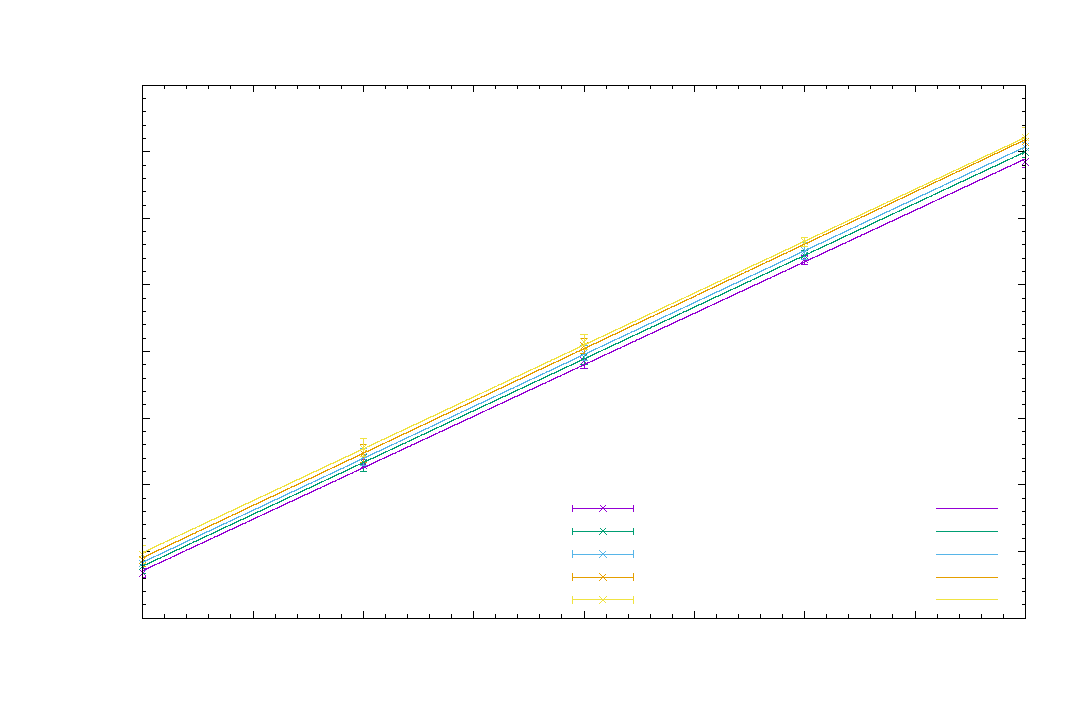
\includegraphics[width={504.00bp},height={324.00bp}]{tv4-l-plus}}%
    \gplfronttext
  \end{picture}%
\endgroup
